% 这是中国科学院大学计算机科学与技术专业《计算机组成原理(研讨课)》使用的实验报告 Latex 模板
% 本模板与 2024 年 2 月 Jun-xiong Ji 完成, 更改自由 Shing-Ho Lin 和 Jun-Xiong Ji 于 2022 年 9 月共同完成的基础物理实验模板
% 如有任何问题, 请联系: jijunxoing21@mails.ucas.ac.cn
% This is the LaTeX template for report of Experiment of Computer Organization and Design courses, based on its provided Word template. 
% This template is completed on Febrary 2024, based on the joint collabration of Shing-Ho Lin and Junxiong Ji in September 2022. 
% Adding numerous pictures and equations leads to unsatisfying experience in Word. Therefore LaTeX is better. 
% Feel free to contact me via: jijunxoing21@mails.ucas.ac.cn

\documentclass[11pt]{article}

\usepackage[a4paper]{geometry}
\geometry{left=2.0cm,right=2.0cm,top=2.5cm,bottom=2.5cm}

\usepackage{ctex} % 支持中文的LaTeX宏包
\usepackage{amsmath,amsfonts,graphicx,subfigure,amssymb,bm,amsthm,mathrsfs,mathtools,breqn} % 数学公式和符号的宏包集合
\usepackage{algorithm,algorithmicx} % 算法和伪代码
\usepackage[noend]{algpseudocode} % 算法和伪代码
\usepackage{fancyhdr} % 自定义页眉页脚
\usepackage[framemethod=TikZ]{mdframed} % 创建带边框的框架
\usepackage{fontspec} % 字体设置
\usepackage{adjustbox} % 调整盒子大小
\usepackage{fontsize} % 设置字体大小
\usepackage{tikz,xcolor} % 绘制图形和使用颜色
\usepackage{multicol} % 多栏排版
\usepackage{multirow} % 表格中合并单元格
\usepackage{pdfpages} % 插入PDF文件
\usepackage{listings} % 在文档中插入源代码
\usepackage{wrapfig} % 文字绕排图片
\usepackage{bigstrut,multirow,rotating} % 支持在表格中使用特殊命令
\usepackage{booktabs} % 创建美观的表格
\usepackage{circuitikz} % 绘制电路图
\usepackage{zhnumber} % 中文序号(用于标题)
\usepackage{tabularx} % 表格折行

\definecolor{dkgreen}{rgb}{0,0.6,0}
\definecolor{gray}{rgb}{0.5,0.5,0.5}
\definecolor{mauve}{rgb}{0.58,0,0.82}
\lstset{
  frame=tb,
  aboveskip=3mm,
  belowskip=3mm,
  showstringspaces=false,
  columns=flexible,
  framerule=1pt,
  rulecolor=\color{gray!35},
  backgroundcolor=\color{gray!5},
  basicstyle={\small\ttfamily},
  numbers=none,
  numberstyle=\tiny\color{gray},
  keywordstyle=\color{blue},
  commentstyle=\color{dkgreen},
  stringstyle=\color{mauve},
  breaklines=true,
  breakatwhitespace=true,
  tabsize=3,
}

% 轻松引用, 可以用\cref{}指令直接引用, 自动加前缀. 
% 例: 图片label为fig:1
% \cref{fig:1} => Figure.1
% \ref{fig:1}  => 1
\usepackage[capitalize]{cleveref}
% \crefname{section}{Sec.}{Secs.}
\Crefname{section}{Section}{Sections}
\Crefname{table}{Table}{Tables}
\crefname{table}{Table.}{Tabs.}

% \setmainfont{Palatino Linotype.ttf}
% \setCJKmainfont{SimHei.ttf}
% \setCJKsansfont{Songti.ttf}
% \setCJKmonofont{SimSun.ttf}
\punctstyle{kaiming}
% 偏好的几个字体, 可以根据需要自行加入字体ttf文件并调用

\renewcommand{\emph}[1]{\begin{kaishu}#1\end{kaishu}}

% 对 section 等环境的序号使用中文
\renewcommand \thesection{\zhnum{section}、}
\renewcommand \thesubsection{\arabic{section}}


%%%%%%%%%%%%%%%%%%%%%%%%%%%
%改这里可以修改实验报告表头的信息
\newcommand{\name}{艾华春, 李霄宇, 王敬华}
\newcommand{\studentNum}{2022K8009916011}
\newcommand{\major}{计算机科学与技术}
\newcommand{\labNum}{3}
\newcommand{\labName}{在流水线中添加普通用户态指令}
%%%%%%%%%%%%%%%%%%%%%%%%%%%

\begin{document}

\begin{center}
  \LARGE \bf 中国科学院大学 \\《计算机体系结构基础(研讨课)》实验报告
\end{center}

\begin{center}
  \emph{姓名} \underline{\makebox[10em][c]{\name}} \\
  % 如果名字比较长, 可以修改box的长度"8em"为其他值
  \emph{学号} \underline{\makebox[30em][c]{\studentNum}}\\
  % \emph{专业} \underline{\makebox[15em][c]{\major}}\\
  \emph{实验项目编号} \underline{\makebox[3em][c]{\labNum}}
  \emph{实验名称} \underline{\makebox[30em][c]{\labName}}\\
\end{center}

% \begin{center}
%   \begin{tabularx}{\textwidth}{|lX|}
%     \hline
%     注1: & 撰写此 Word 格式实验报告后以 PDF 格式保存 SERVE CloudIDE 的 \texttt{/home/serve-ide/ cod-lab/reports} 目录下(注意:reports 全部小写)。文件命名规则:\texttt{prjN.pdf},其中 \texttt{prj} 和后缀名 \texttt{pdf} 为小写,\texttt{N} 为1至4的阿拉伯数字。例如:\texttt{prj1.pdf}。PDF 文件大小应控制在 5MB 以内。此外,实验项目5包含多个选做内容,每个选做实验应提交各自的实验报告文件,文件命名规则:\texttt{prj5-projectname.pdf},其中``-''为英文标点符号的短横线。文件命名举例:\texttt{prj5-dma.pdf}。具体要求详见实验项目5讲义。 \\

%     注2: & 使用\texttt{git add}及\texttt{git commit}命令将实验报告\texttt{PDF}文件添加到本地仓库master分支,并通过\texttt{git push}推送到实验课SERVE GitLab远程仓库master分支(具体命令详见实验报告)。 \\

%     注3: & 实验报告模板下列条目仅供参考,可包含但不限定如下内容。实验报告中无需重复描述讲义中的实验流程。\\
%     \hline
%   \end{tabularx}
% \end{center}

  

\section{逻辑电路结构与仿真波形的截图及说明}

\noindent
$\bullet$
\textbf{访存指令添加}。
\begin{enumerate}
  \item 添加访存操作类型的数据通路
  
  在ID(译码)阶段添加判断当前的load 或 store操作的类型,包括是否无符号扩展,数据的位宽。并将相应的信号沿着流水级传递到MEM(访存)阶段。

  \begin{lstlisting}[language=verilog]
    assign id_op_st_ld_b      = op_25_22[1:0] == 2'd0;    // 位宽为1 byte
    assign id_op_st_ld_h      = op_25_22[1:0] == 2'd1;    // 位宽为2 byte
    assign id_op_st_ld_u      = op_25_22[3];              // 无符号数扩展
  \end{lstlisting}
\item 添加从EX到MEM访存地址最低两位传递数据通路

  在EX到MEM的传递的数据中添加访存地址的最低两个bit,使得MEM阶段可以获取到从sram中取出来1字节的数据内部的偏移。

  \item 在load操作的结果处添加多路选择器(在访存流水级)
  
  首先,通过操作的数据位宽和访存地址来选择出从sram中输出的的数据的有效部分。
  \begin{lstlisting}[language=verilog]
    // mem_data_sram_addr[2] 是上一小节中传递过到mem级的访存地址后两位
    assign mem_word_result =    data_sram_rdata;   // ld.w 的有效部分
    assign mem_half_result =    mem_data_sram_addr[1] ? data_sram_rdata[31:16]
                                : data_sram_rdata[15:0];    // ld.h 的有效部分
    assign mem_byte_result =    ({8{mem_data_sram_addr[1:0] == 2'd0}} & data_sram_rdata[7:0])
                                |({8{mem_data_sram_addr[1:0] == 2'd1}} & data_sram_rdata[15:8])
                                |({8{mem_data_sram_addr[1:0] == 2'd2}} & data_sram_rdata[23:16])
                                |({8{mem_data_sram_addr[1:0] == 2'd3}} & data_sram_rdata[31:24]);
                                // ld.b 的有效部分

  \end{lstlisting}

  然后根据有符号扩展还是无符号数扩展,对结果进行扩展,最终得到可以写入目的寄存器(rd)的结果\verb|mem_result|。
  \begin{lstlisting}[language=verilog]
    // mem_op_st_ld_b, mem_op_st_ld_h 分别表示数据位宽为1byte和2byte
    // mem_op_st_ld_u 表示数据进行无符号数扩展(即0扩展)
    // ~mem_op_st_ld_u & mem_byte_result[7]  或~mem_op_st_ld_u & mem_half_result[15] 表示符号位
    assign mem_result 
    = mem_op_st_ld_b ? ({{24{~mem_op_st_ld_u & mem_byte_result[7]}}, mem_byte_result[7:0]}):       
      mem_op_st_ld_h ? ({{16{~mem_op_st_ld_u & mem_half_result[15]}}, mem_half_result[15:0]}) :
      mem_word_result;
  \end{lstlisting}

  \item 在store操作中传递给\verb|data_sram|的信号处添加选择器
  
  首先,根据访存的位宽和地址,通过多路选择和移位操作确定字节使能信号。
  \begin{lstlisting}[language=verilog]
    // 字节使能
    // st.b 时,根据访存地址的最低两位进行移位操作。有四种不同情况
    // st.h 时,根据访存地址的最低两位添加二选以选择器。有两种不同情况
    assign ex_sram_we = ex_op_st_ld_b ? (4'b0001 << ex_data_sram_addr[1:0]) :           // st.b
                      ex_op_st_ld_h ? (ex_data_sram_addr[1] ? 4'b1100 : 4'b0011) :    // st.h
                      4'b1111;                                    // st.w
  \end{lstlisting}
  确定字节使能后,生成写入数据。不需要将数据进行移动,而是仅仅根据数据长度,对有效部分进行赋值连接操作,
  确保数据在写入时能拿到有效的数据。
\begin{lstlisting}[language=verilog]
  //生成写入数据
  //对有效部分进行赋值连接操作
  assign data_sram_wdata  =    ex_op_st_ld_b ? {4{ex_rkd_value[7:0]}}:
                              ex_op_st_ld_h ? {2{ex_rkd_value[15:0]}}:
                              ex_rkd_value[31:0];
\end{lstlisting}
\end{enumerate}


\vspace{1ex}

\section{实验过程中遇到的问题、对问题的思考过程及解决方法(比如RTL代码中出现的逻辑bug,逻辑仿真和FPGA调试过程中的难点等)}

\noindent
$\bullet$
\textbf{data_sram写使能bug}。
在仿真中,在load指令中,写入寄存器的结果与标准结果不一致。

然后在波形图中查看从sram直接返回的数据,发现同样与标准结果不一致,于是排除是新添加的load多路选择器的问题。

进而在反汇编代码中,发现在load指令前,有一条store指令,地址相同。于是在波形图中查看相关波形,发现该指令ex阶段的sram写使能没有拉高,再回溯到id阶段,
发现是mem写使能中,不同种类的load之间的逻辑连接错写成与,导致不能向sram写入数据。

\begin{lstlisting}[language=verilog]
//  assign id_mem_we        = inst_st_w & inst_st_b & inst_st_h & id_valid;  
assign id_mem_we        = (inst_st_w | inst_st_b | inst_st_h) & id_valid;  
\end{lstlisting}
\vspace{1ex}

\noindent
$\bullet$
\textbf{ALU设计问题}。
请输入你的实验报告内容。

如果一段话写不下,可以再这里继续新的段落。

插入图片,可以参考如下方法:
\begin{figure}[h]
  \centering
  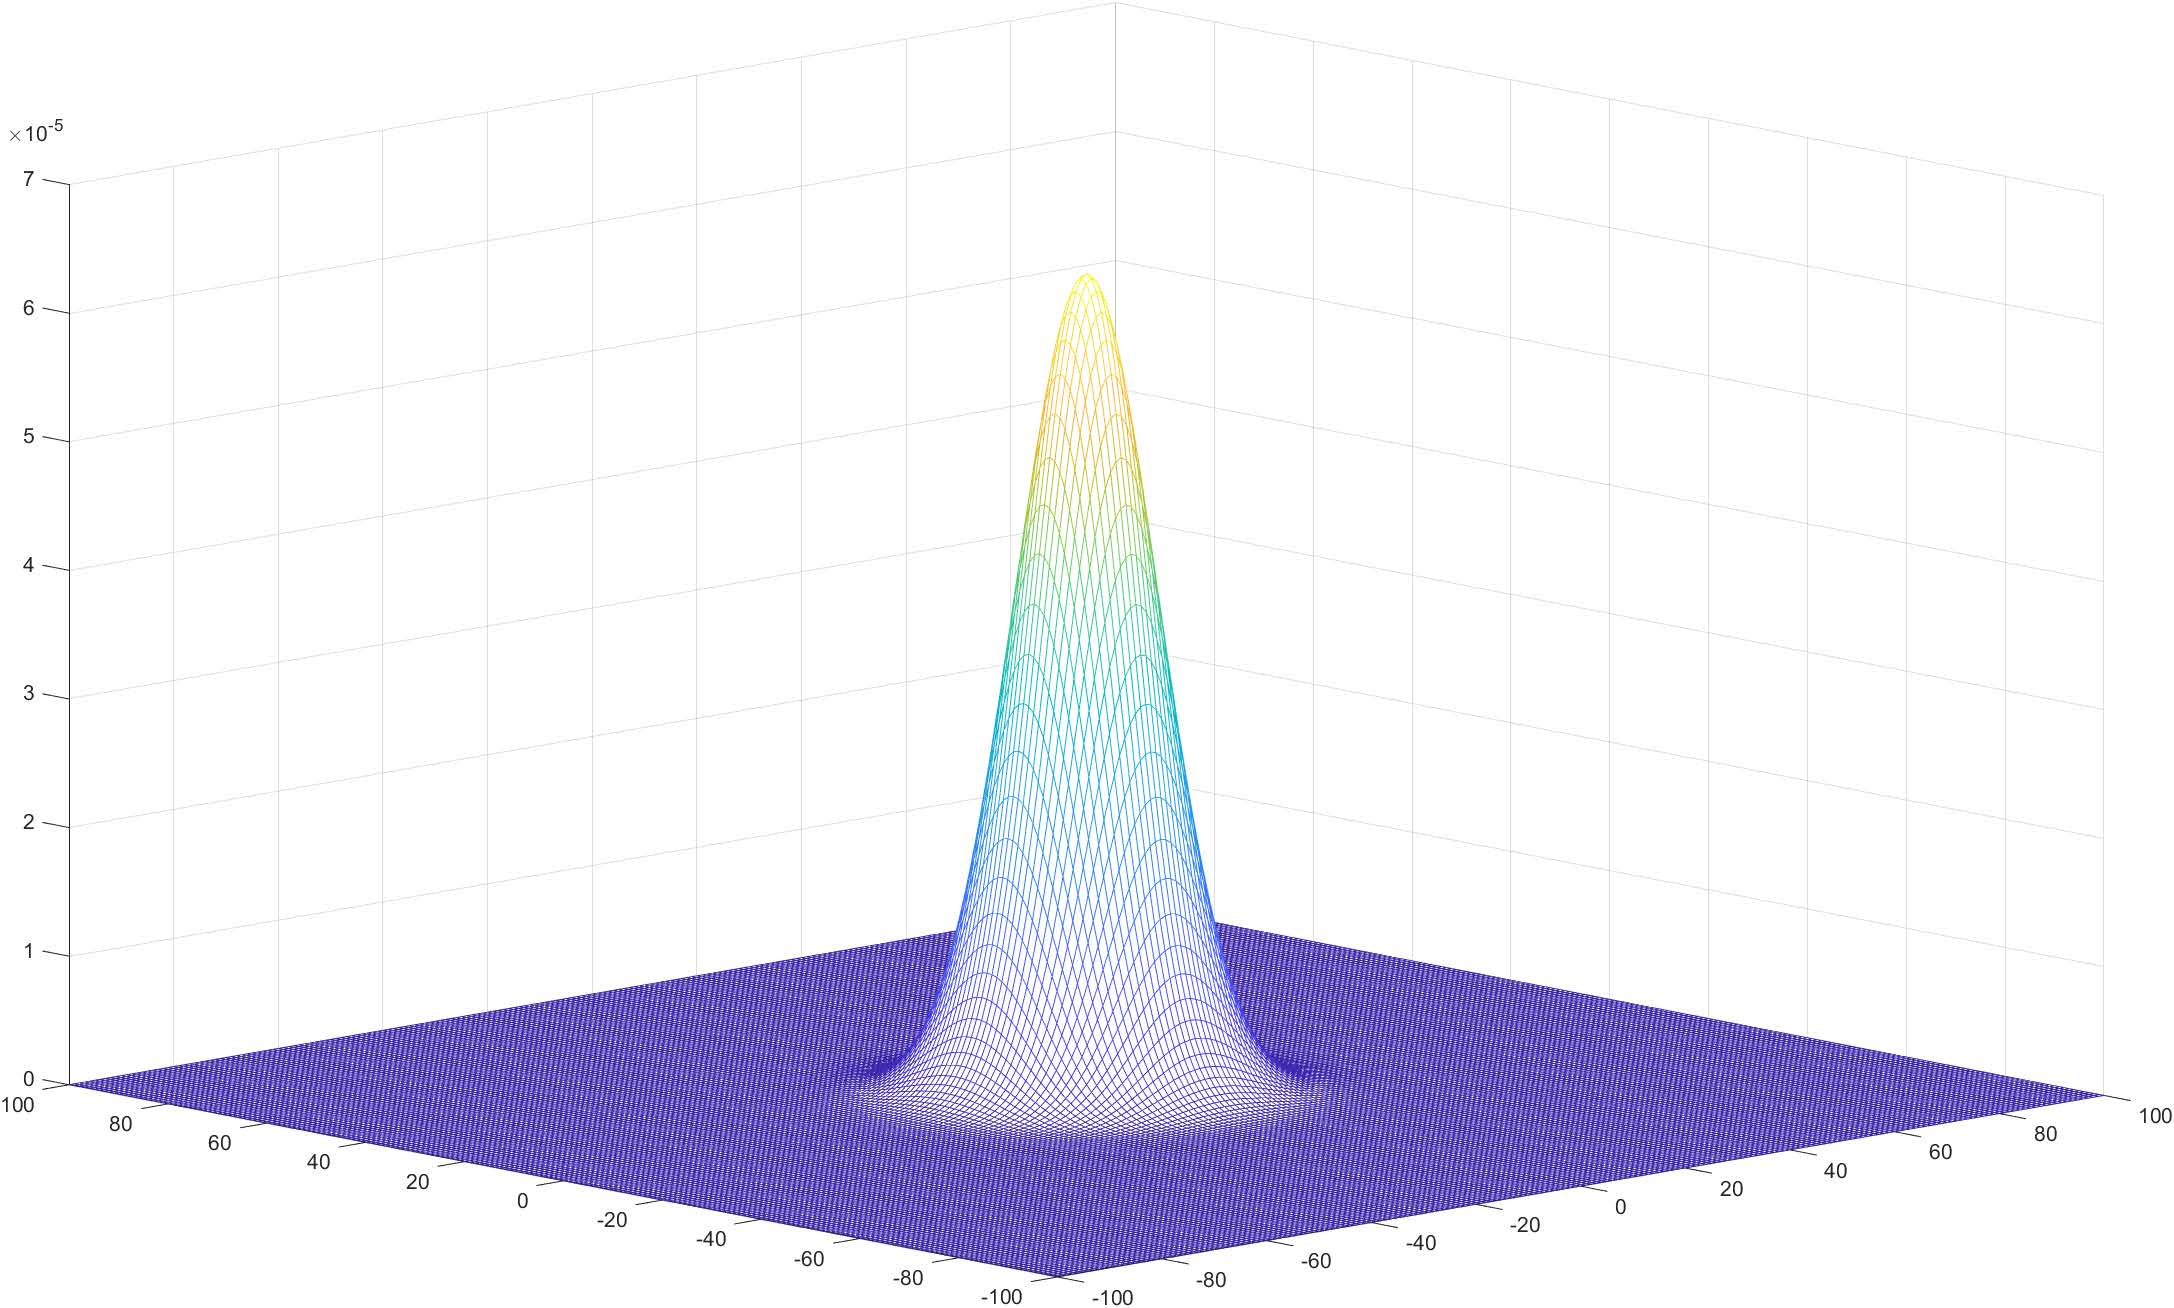
\includegraphics[width=10cm]{fig/Gaussian.pdf}
  \caption{这是第一张图}
\end{figure}

\vspace{1ex}

\noindent
$\bullet$
\textbf{其他关键模块设计问题}。
请输入你的实验报告内容。

如果一段话写不下,可以再这里继续新的段落。

插入第二张图片:
\begin{figure}[h]
  \centering
  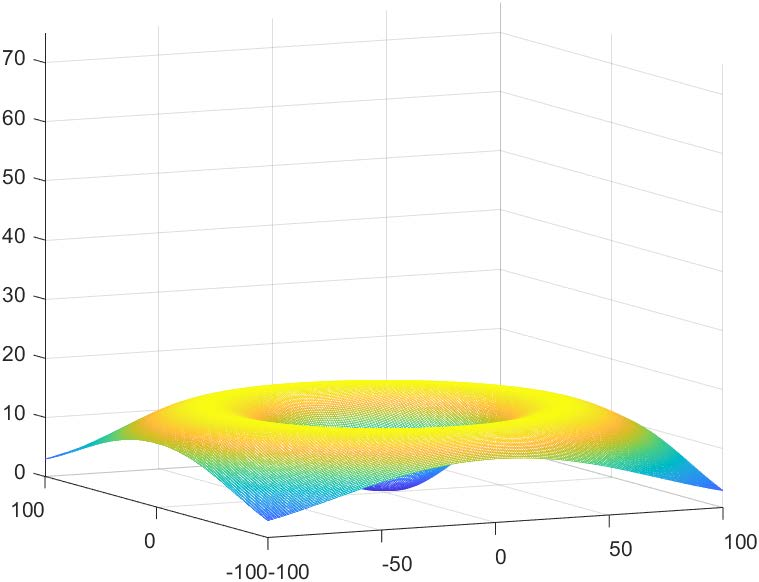
\includegraphics[width=10cm]{fig/Maxwell.pdf}
  \caption{这是第二张图}
\end{figure}

\end{document}